%%%%%%%%%%%%%%%%%%%
% SECTION: VGG Face
%%%%%%%%%%%%%%%%%%%
\section{Pre-Trained Models}

\subsection{VGG Face}

The VGG-Face neural network is a CNN designed and implemented by Parkhi, Vedaldi and Zisserman \cite{Parkhi2015DeepRecognition} from the University of Oxford. The CNN descriptors are computed using a CNN based on the VGG16 which are evaluated on the Labelled Faces in the Wild \cite{HuangLabeledEnvironments} and the YouTube Faces \cite{WolfFaceSimilarity} datasets. The input of the CNN must be a face image of size 224x224. The VGG-Face consists of 18 layers consisting of convolutional layers, pooling layers, and activation layers. The 18 layers make up 11 blocks, out of which, the first eight blocks are Convolutional layers followed by non-linearities such as ReLU and max pooling. The last three blocks are Fully Connected layers (FC) \cite{Parkhi2015DeepRecognition}. An overview of the VGG-Face is shown in figure \ref{fig:vggarchitecture}. The full detail of the network's architecture is shown in table \ref{table:vggface}.

% FIGURE: vgg architecture
\begin{figure}[H]	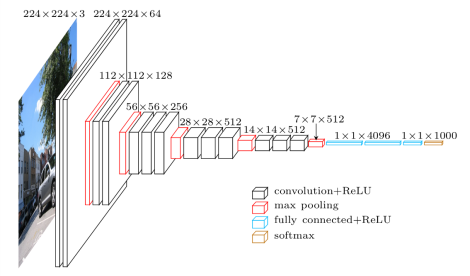
\includegraphics[width=0.8\linewidth]{images/vggarchitecture.png} 
\centering

\caption{VGG-Face Architecture.} 

\label{fig:vggarchitecture}
\end{figure}

Several choices for the VGG-Face were chosen to run the following experiments. The first choice is to add or remove the three Fully Connected layers at the end of the CNN. If the three Fully Connected layers when these layers where not added, there were two other options. The first option is to use pooling for feature extraction to the output of the last convolutional layer. Either an average global pooling or a maximum global pooling can be used, both options are explored. The last option is not to use any of layer after the last Convolutional layer.

% FIGURE: vgg face
\begin{figure}[h]	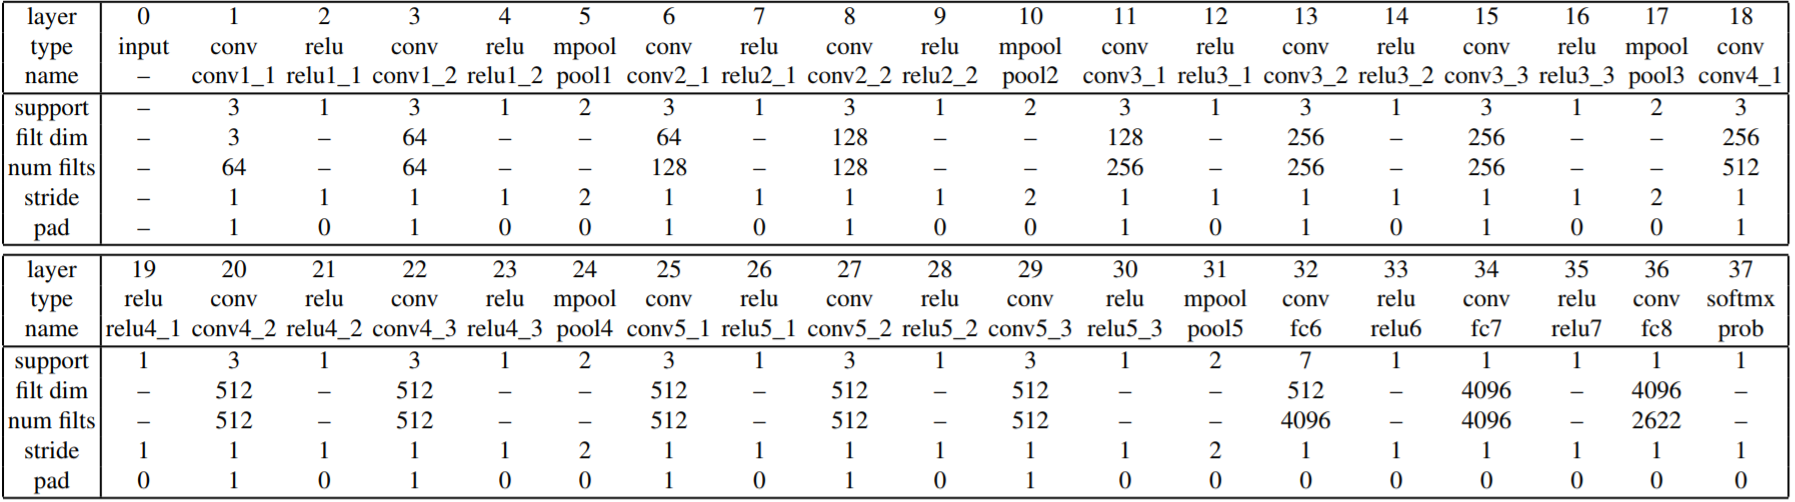
\includegraphics[width=\linewidth]{images/vggface.png} 
\caption{Fully connected layers are listed as convolutional layers. Each convolution has it's corresponding padding, number of filters and stride. \cite{Parkhi2015DeepRecognition} } 
\label{table:vggface}
\end{figure}

%%%%%%%%%%%%%%%%%%%
% SECTION: C3D Model
%%%%%%%%%%%%%%%%%%%
\subsection{C3D Model}

\textbf{C3D} is a 3D CNN model introduced by Tran et al. \cite{Tran2015LearningNetworksb} that is able to learn spatio-temporal features. The model architecture, presented in figure \ref{fig:c3d_architecture}, consists of 8 convolution, 5 max-pooling, and 2 fully connected layers, followed by a softmax output layer. 

% FIGURE: C3D architecture
\begin{figure}[!htb]	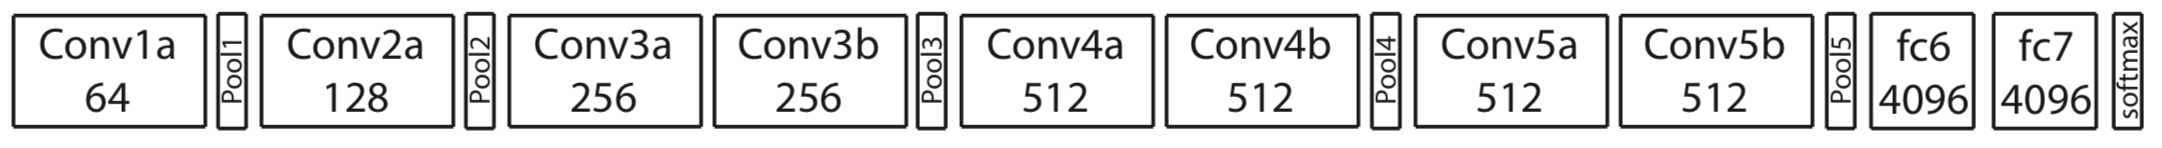
\includegraphics[width=0.9\textwidth]{images/c3d_architecture.png} 
    \centering

\caption{
C3D Architecture. \cite{Tran2015LearningNetworks}
} 

\label{fig:c3d_architecture}
\end{figure}

All 3D convolution kernels are 3 × 3 × 3 with stride 1 in both spatial and temporal dimensions. Number of filters are denoted in each box. The 3D pooling layers are denoted from pool1 to pool5. All pooling kernels are 2 × 2 × 2, except for pool1 is 1 × 2 × 2. Each fully connected layer has 4096 output units.

The C3D model code implementation used in this thesis was taken from Alberto Montes github project (github.com/albertomontesg). Monte's implementation is a Keras \cite{Chollet2015Keras} model, converted from the original Caffe \cite{JiaCaffe:} implementation by Tran et al. \cite{Tran2015LearningNetworks} for large-scale video classification. \cite{Karpathy2014Large-scaleNetworks}